\documentclass[pdftex,a4paper,titlepage,11pt]{article}
\usepackage[T1]{fontenc}
\usepackage[utf8]{inputenc}
\usepackage[english,francais]{babel}
\usepackage{listings}
\usepackage{setspace}

\usepackage[top=2.5cm, bottom=2.5cm, left=3.0cm, right=3.0cm, a4paper]{geometry}

\usepackage{avant}
\usepackage{fancyvrb}
\usepackage{fancyhdr}
\pagestyle{fancy}
\fancyhf{}
\fancyhead[RO]{\itshape\thepage}
% \fancyhead[LO]{\itshape\rightmark}
% \fancyhead[RE]{\itshape\leftmark}
\renewcommand{\headrulewidth}{0.5pt}

% \addtolength{\headheight}{0.5pt}
% \renewcommand\footrulewidth{0pt}
\fancypagestyle{plain}{
    \fancyhead{}
    \renewcommand{\headrulewidth}{0pt}}
\usepackage{textcomp}
\usepackage{relsize}
\usepackage{amssymb}
\usepackage[colorlinks=true,linkcolor=black,citecolor=black,urlcolor=black,filecolor=black]{hyperref}
\usepackage{framed}
\usepackage[pdftex]{graphicx}
\usepackage{makeidx}
% \addtolength{\textwidth}{1cm}
% \setlength{\textheight}{24cm} 	% Hauteur de la zone de texte

%%%%%%%%%%%%%%%%%%%%%%%%%%%%%%%%%%%%%%%%%%%%%%%%%%%%%%%

\newcommand{\executeiffilenewer}[3]{%
 \ifnum\pdfstrcmp{\pdffilemoddate{#1}}%
 {\pdffilemoddate{#2}}>0%
 {\immediate\write18{#3}}\fi%
}

\newcommand{\includesvg}[2]{%
 \executeiffilenewer{#1.svg}{#1.pdf}%
 {inkscape -z -D --file=#1.svg --export-pdf=#1.pdf --export-width=1000}%
 %\input{#1.eps_tex}%
 \includegraphics[scale=#2]{#1.pdf}
}

\newcommand{\includedot}[2]{%
 \executeiffilenewer{#1.dot}{#1.pdf}%
 {dot -T pdf -o #1.pdf #1.dot}%
 %\input{#1.eps_tex}%
 \includegraphics[scale=#2]{#1.pdf}
}

\newcommand{\includepic}[2]{%
 \immediate\write18{pic2plot -Tsvg --bg-color none #1.pic > #1.svg && inkscape -z -D --file=#1.svg --export-pdf=#1.pdf --export-width=1000}%
 \includegraphics[scale=#2]{#1.pdf}
}

%%%%%%%%%%%%%%%%%%%%%%%%%%%%%%%%%%%%%%%%%%%%%%%%%%%%%%%

% nouvelle commande pour un joli nom
\newcommand{\nom}[1]{\textsc{#1}}

% commande pour une zolie ligne
\newcommand{\ligne}[1][1pt]{
  \par\noindent
  \rule[.5ex]{\linewidth}{#1}\par}

% nettoyer une page blanche avant une page de chapitre en mode openright
\newcommand{\clearemptydoublepage}{
	\newpage{\pagestyle{empty}\cleardoublepage}}


\makeindex

\begin{document}

% augmenter l'espacement entre plusieurs paragraphes plutôt que de passer des lignes quand il faut pas
\setlength{\parskip}{2.4ex}

\title{
\ligne{\Large}
\textbf{Contextd Capture}\\
\textbf{Project de deuxième année}\\
\Large Capture d'activité système pour PIGA-SYSTRANS
% \Large Généralisation des plugins de communication avec contextd
\ligne{\Large}
}
\author{\nom{Dimitri Gressin} \& \nom{Timothée Ravier}\\\\\nom{Pilote : Jérémy Briffaut}}
\date{27 \textsc{mai} 2011}

% titre
\maketitle

% page blanche
\clearemptydoublepage

% table des matières
\setcounter{secnumdepth}{3}
\setcounter{tocdepth}{2}
\addtocontents{toc}{\protect\thispagestyle{empty}}
\tableofcontents
\addtocounter{page}{-1}

\newpage

\section*{Introduction} \addcontentsline{toc}{section}{Introduction}
Ce rapport présente le travail et les résultats obtenus dans le cadre de notre projet d'application de deuxième année. Ce projet s'inscrit dans le cadre des projets de recherche menés au Laboratoire d'Informatique Fondamentale d'Orléans (LIFO) par l'équipe Sécurité et Distribution des Systèmes (SDS) sur la création d'un système d'exploitation sécurisé basé sur Linux.
% FIXME Est-ce correct ?

~

Ce projet a pour but la simplification et la généralisation du contrôle d'application par le démon contextd. Contextd est un démon résident en espace utilisateur qui commande et coordonne différents systèmes de sécurité (SELinux, PIGA-MAC, iptables...). Il permet de changer dynamiquement la configuration de ces outils de sécurité pour assurer la sécurité et la cohérence globale d'un système. Il constitue une mise en oeuvre avancée du principe de séparation des privilèges, limitant les droits des applications contrôlées au strict minimum, à chaque instant donné.

~

Mais pour fonctionner, Contextd doit avoir connaissance des actions entreprisent par chacune des applications que l'on veut surveiller. Jusqu'à présent, la communication entre les applications et contextd s'effectuait via un pluging ou un patch propre à chaque application. Contextd recueillait alors les demandes de chacunes de ces applications (lecture/écriture de fichiers, création de socket...) pour en déduire un domaine (web, ecommerce, mail...). Contextd était donc limité aux informations fournies par ces applications.

~

L'idée retenue consiste à déplacer la contrainte de communication au niveau du noyau, qui par l'intermédiaire des appels système a connaissance des actions effectuées par les programmes. Il s'agit donc de modifier le fonctionnement du noyau Linux ainsi que le comportement de contextd et la nature de ses sources d'information.

~

\newpage

\section{\'Etat de l'art}

Ce projet de deuxième année s'inscrit dans le contexte de la sécurité d'un système d'exploitation. La majeur partie des systèmes d'exploitation actuels ont intégré une forme de contrôle d'accès pour assurer un minimum de sécurité et de contrôle sur les activités des utilisateurs, dans le but de limiter les effets d'une attaque sur un système. Dans les faits, ce contrôle n'est pas suffisant et ne peut empêcher, par exemple, la compromition d'un système par l'intermédiaire d'un service possédant les droits d'administrateur \cite{TIOF}, ou l'échange d'information par flux indirects, comme des fichiers temporaires.

Plus généralement, c'est dans l'absence de mécanisme de sécurité global imposé à un système que réside les manques des modèles de sécurité classique. Plus que simplement le noyau et les applications, ce sont l'ensemble des intéractions entre tous ces éléments qui doivent être contrôlées. Nous allons détailler les différents objectifs à atteindre avant de poursuivre sur les modèles théoriques et leur implémentation dans les systèmes d'exploitation modernes.

%  Nous allons détailler les objectifs à atteindre avant de présenter les différentes solutions disponibles.
% Il existe différents mécanismes qui permettent d'apporter des couches de sécurité à un tel système. Nous détaillerons donc les principes fondateurs de la sécurité pour enchaîner sur les solutions disponibles.

Nous allons réduire les concepts d'utilisateurs et d'applications aux ``simples'' processus qui sont la base de toute intéraction avec un système. De même, les fichiers, sockets, les IPC sont autant d'éléments sur lesquel un processus peut agir et nous les regrouperons sous le terme d'objet.

\subsection{Les objectifs de sécurité}

La sécurité d'un système d'information et plus particulièrement la sécurité des systèmes d'exploitation réside dans l'application de mesures visant à atteindre les objectifs suivants :

\textbf{Confidentialité :}
Les informations ne doivent être accessibles qu'aux utilisateurs qui en ont besoin et qui disposent des privilèges correspondant. Il ne doit notamment pas être possible de transmettre de l'information confidentielle à un niveau inférieur.

\textbf{Intégrité :}
Le système reste dans un état cohérent. Les informations importantes comme les mots de passe, les binaires installés, les fichiers de configuration ne peuvent être modifiés par des utilisateurs non privilégiés.

\textbf{Disponibilité :}
Le système doit être réactif, stable et utilisable. Les programes doivent pouvoir fonctionner correctement. Les contrôles de sécurité supplémentaires instaurés ne doivent pas limiter les capacités légitimes du système et des applications.

\textbf{Authenticité :}
Il est possible de savoir qui a effectué quelle action critique sur un système.

\textbf{Non-répudiation :}
L'origine et le contenu de certaines informations ne peut être mis en doute. Cela permet par exemple de s'assurer de l'enregistrement des comportements suspects sur une machine, ou de valider l'origine de certaines données.

\subsection{Le principe de séparation des privilèges}

Une des technique utilisée pour tenter d'atteindre ces objectifs consiste à appliquer le principe de séparation des privilèges ou principe de moindre privilège. Il stipule qu'un programme (contrôlé ou non par l'utilisateur) ne doit disposer que des droits strictement nécessaire à son bon fonctionnement. Par exemple, il semble évident qu'un logiciel de traitement de texte n'a pas besoin d'avoir accès aux informations sensibles du système comme la liste des utilisateurs ou la liste des mots de passe.

L'application la plus courante de ce principe est la séparation entre les différents comptes sur un système. Une application lancée par un utilisateur ne bénéficie que des droits accordés à cet utilisateur.

\subsection{A qui faire confiance ?}

Il est possible d'employer différentes approches pour s'assurer de la sécurité d'un système d'exploitation, mais chacune d'entre elles repose à un moment ou un autre sur la confiance que l'on a dans l'un des éléments qui la constitue. On peut citer plusieurs cas de figures \cite{WCS}:

\begin{itemize}
  \item Faire confiance à tous les logiciels à propos du respect de la politique de sécurité, tout en étant conscient que les logiciels ne sont pas de confiance % Trust all the software to abide by a security policy but the software is not trustworthy (this is computer insecurity).
  \item Faire confiance à tous les logiciels à propos du respect de la politique de sécurité et s'assurer que le logiciel est validé et fiable (analyse complète et exhaustive de tous les cas d'utilisations, de toutes les branches du code) % Trust all the software to abide by a security policy and the software is validated as trustworthy (by tedious branch and path analysis for example).
  \item Ne faire confiance à aucun programme, mais imposer une politique de sécurité même si la fiabilité de cette politique et son moyen d'application n'est pas complétement fiable% enforce a security policy with mechanisms that are not trustworthy (again this is computer insecurity).
  \item Ne faire confiance à aucun programme, mais s'assurer qu'une politique de sécurité est appliquée par des méchanismes matériels de confiance% trustworthy hardware mechanisms. %FIXME
\end{itemize}

Les modèles de sécurité standard se situent tous dans la première catégrie alors que les méthodes que nous allons présenter par la suite peuvent être placées dans les catégories trois et quatre. Le test complet de tous les logiciels présents sur un système d'exploitation est une tâche difficilement réalisable si l'on considère la diversité des matériels disponibles et la complexité d'une application telle que le noyau d'un système d'exploitation. Il existe des systèmes d'exploitation et plus particulièrement des noyaux certifiés critères communs, tel QNX\cite{QNX}, qui peuvent être classés dans la catégorie 2. En revanche, le code source de ces différents systèmes n'étant pas disponible librement, nous ne les détaillerons pas dans ce document.

\subsection{Les différentes méthodes de contrôle d'accès}

Pour atteindre les objectifs détaillés précédement et assurer la séparation des privilèges, nous allons détailler dans cette partie plusieurs méthodes de contrôle d'accès.

\subsubsection{Contrôle d'accès discrétionnaire (DAC)}

Le contrôle d'accès discrétionnaire correspond à un modèle laissant à l'utilisateur, et donc aux programmes qu'il lance, tout contrôle sur les droits accordés aux objets qu'il possède. Un utilisateur peut ainsi compromettre un système en accordant des droits importants à d'autres utilisateurs sur les fichiers qu'il possède. Ce modèle ne permet pas d'assurer la confidentialité, l'intégrité d'un système. Il est à ranger dans la première catégorie des modèles qui font confiance aux logiciels sans imposer de contrôle de sécurité fort.

\subsubsection{Contrôle d'accès mandataire (MAC)}

Le contrôle d'accès mandataire repose sur la séparation entre les applications et l'entité prenant la décision d'autoriser ou d'interdire une action. Cette entité peut être implémentée au sein du noyau ou à l'aide de mécanismes externes au système, éventuelement matériels \cite{ITXT}. Ce modèle permet d'assurer la conformité du système à un ensemble de règles qui foment une politique de sécurité. Il est ainsi possible d'appliquer le principe de moindre privilèges en partant d'une base n'autorisant aucune intéraction puis en rajoutant progressivement des intéractions autorisées. Le contrôle d'accès mandataire correspond aux catégories trois et quatre, oû l'on ne fait pas confiance aux applications pour se reposer sur l'application d'une politique de sécurité plus ou moins fiable.

% \begin{figure}[h]
% 	\centering
% 	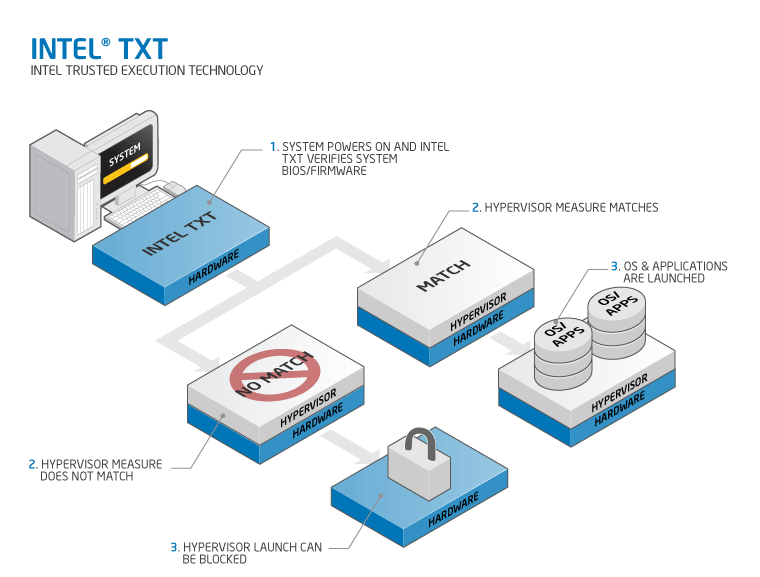
\includegraphics[scale=0.70]{attachements/techrefresh-info-txtfull.png}
% 	\caption{Intel Trusted Execution Technology}
% \end{figure}

\subsubsection{Sécurité multiniveau, multi catégorie (MLS ou MCS)}

Le modèle de sécurité multiniveau permet d'atteindre certains des buts fixés comme l'intégrité ou la confidentialité. Il repose sur la séparation des données en plusieurs domaines, imposant des règles limitant les intéractions de l'utilisateur.

\textbf{Bell-LaPaluda :} Ce modèle préserve la confidentialité de l'information en n'autorisant un sujet à écrire uniquement dans un niveau de confidentialité supérieur ou égal, et à ne lire que dans un niveau de sécurité inférieur ou égal. Ce modèle présente plusieurs inconvénients majeurs parce qu'il ne permet pas d'imposer des contraintes d'intégrité et ne permet pas de faire de disctinctions précise entre deux personnes possédant le même niveau d'accréditation.

\begin{figure}[h]
	\centering
	\includesvg{attachements/bell-lp}{0.45}
	\caption{Le modèle Bell-LaPadula}
\end{figure}

\textbf{Biba :} A contrario du modèle précédent, c'est l'intégrité qui est préservée, car seules les modifications dans un niveau de sécurité inférieur sont autorisée, et la lecture ne peut se faire que sur un niveau d'intégrité supérieur.

\begin{figure}[h]
	\centering
	\includesvg{attachements/biba}{0.45}
	\caption{Le modèle Biba}
\end{figure}

Ces deux modèles ne permettent pas d'atteindre plus d'un ou deux objectifs à la fois, et posent le problème de la sur-classification des données (toutes les données devenues confidentielles). Ceci conduit à l'introduction d'une méthode de déclassification, compromettant l'ensemble du modèle.

\subsubsection{Contrôle d'accès basé sur des rôles (RBAC)}

Plus qu'un modèle réel de contrôle, c'est un modèle d'administration permettant de simplifier le travail de l'administrateur d'un système utilisant un contrôle mandataire. Le principe du contrôle d'accès mandataire consiste à attribuer des rôles à chaque utilisateur de la machine. Ces rôles donnent ainsi accès à différents éléments du système. Par exemple, les rôles d'utilisateur, d'administrateur et de webmaster peuvent être définis et un utilisateur classique pourra se voir attribuer le rôle de webmaster lui autorisant de modifier les pages disponibles sur un serveur sans avoir besoin de donner un accès administrateur complet à cette personne.

\subsubsection{Application de règles de politiques securité par les types (Type Enforcement)}

Ce principe repose sur l'association d'un contexte de sécurité à chaque objets et processus. L'accès à un object par un processus doit correspondre à une règle de la politique de sécurité pour être autorisé. Ce modèle nécessite l'attribution d'un contexte de sécurité à tous les objets du système, y compris les fichiers présents sur les supports de stockage.

\subsection{Solutions disponibles}

Nous allons détailler les implémentations de ces modèles de sécurité dans certains systèmes d'exploitations, notamment les systèmes ``libres'', pour lesquels nous pouvons avoir accès au code source : Linux et la famille des BSD.

\subsubsection{SELinux}

SELinux est une implémentation d'un mécanisme de contrôle d'accès mandataire basé sur le ``type enforcement'', de niveau de sécurité/confidentialité non prédéfinis, et d'un contrôle d'accès basé sur les rôles. SELinux a été développé par la National Security Agency (NSA) et a été intégrée au noyau Linux une fois que l'architecture des Linux Security Modules fut mise en place. SELinux permet de contrôler à chaque appel système la validité de l'interaction par rapport aux définitions d'une politique. On associe à chaque objets et processus un context de sécurité. L'accès à un object par un processus doit correspondre à une règle de la politique SELinux pour être autorisé. Il faut noter que chaque décission est prise indépendamment des précédantes : SELinux n'as pas de mémoire des transitions effectuées sur un système. C'est cette limitation et la possibilité d'utiliser les flux d'informations indirects, donc non contrôlés par SELinux, qui ont poussé la création de PIGA.

\begin{list}{}{}
 \item \textbf{Contrainte pour l'administrateur :} Il faut décrire la totalité des intéractions possibles pour chaque programme présent sur un système. Il faut s'assurer du bon fonctionnement de ces politiques. Il n'existe pas d'outils pour valider les politiques SELinux. Seuls certains systèmes de fichiers supportent les attributs étendus nécessaires à la labelisation des fichiers présents sur les supports de stockage.
 \item \textbf{Avantages :} Séparation fine des privilèges et des rôles, intégrée dans le noyau. Des politiques ont déjà été écrites. Il existe une distribution facilitant le déploiement de ce type de protection : Fedora.
\end{list}

\subsubsection{PIGA}

L'ensemble désigné sous le nom de PIGA est le résultat de la thèse de Jérémy Briffaut ainsi que des contributions de l'équipe SDS du LIFO, et des étudiants de l'ENSIB. Il est constitué notement d'une surcouche à SELinux permettant de définir et imposer des propriétés de sécurité à l'echelle du système en plus des contrôles au niveau des intéractions effectués par SELinux. Il apporte une ``mémoire'' à SELinux. Un tel résultat est obtenu après génération du graphe complet des intéractions possibles et autorisées par une politique SELinux, recherche de chemins interdits, et consignation de ces chemins. Cette solution permet un contrôle plus avancé sur les flux d'information dans un système, qu'ils soient directs ou indirects.

\begin{list}{}{}
 \item \textbf{Contrainte pour l'administrateur :} Connaissance du langage de définition de propriété PIGA, maîtrise préalable de SELinux, prérequis matériels pour la ``compilation'' des politiques.
 \item \textbf{Avantages :} Un contrôle très fin sur les intéractions dans un système, restriction (statique) des privilèges maximale.
\end{list}

Le système d'exploitation PIGA-OS basé sur la recherche effectué sur PIGA a été vainqueur du concours Sec\&Si organisé par l'Agence Nationale pour la Recherche (ANR) \cite{PIGA}\cite{PIGA2}.

\subsubsection{grsecurity \& PaX}

\textsc{grsecurity} est une autre implémentation des mécanismes de contrôle d'accès mandataire et des listes de contrôle d'accès. Il permet aussi une gestion des droits basée sur les rôles. Souvent associé à \textsc{grsecurity}, PaX est un patch pour le noyau Linux ajoutant des restrictions et des contrôles sur les accès à la mémoire.

\begin{list}{}{}
 \item \textbf{Contrainte pour l'administrateur :} Certains programmes ne fonctionnent plus avec les restrictions implémentées par PaX.
 \item \textbf{Avantages :} Protection avancée de l'utilisation de la mémoire avec PaX (pile non exécutable, ...)
\end{list}

\subsection{TrustedBSD}

% TODO

\subsubsection{iptables}

iptables et un logiciel permettant de contrôler plus facilement netfilter, le parre-feu intégré au noyau Linux. Il permet entre autre de définir précisément quels ports et quelles intéractions avec le réseau sont autorisées sur une machine. Les règles iptables peuvent être modifiées dynamiquement pour autoriser ponctuellement une application à communiquer avec l'extérieur mais le comportement d'iptables est statique par défaut. iptables est un parre-feu à états, c'est à dire qu'il garde en mémoire les intéractions précédantes opur déterminer la légitimité des interactions suivantes.

\begin{list}{}{}
 \item \textbf{Contrainte pour l'administrateur :}
 \item \textbf{Avantages :}
\end{list}

\subsubsection{PIGA-SYSTRANS ou contextd}

contextd est un démon chargé de coordonner différents mécanismes de sécurité sur un système Linux. En effet, dans toutes les solutions décrites préédement, les programmes se voyaient attribués les droits dont ils avaient besoin pour toujours. Une application utilisant ponctuellement le réseau se voyait attribué le droit définitif d'utiliser un port.

\begin{list}{}{}
 \item \textbf{Contrainte pour l'administrateur :}
 \item \textbf{Avantages :}
\end{list}

% TODO & FIXME
% Pax = sécurité automatique
% SELinux, GrSec = MAC qui contrôle les accès directs
% PIGA = contrôle les accès indirects
% iptables contrôle le trafic réseau
% 
% contextd = chef d'orchestre + changement dynamique des règles des autres  mécanismes de protection pour adapter les permissions au domaine d'utilisation.
% 
% Chercher tous les systèmes de MAC/DAC/RBAC,...
% 
% Classer les MAC en fonction du travail à faire par l'administrateur ? en fonction d'où ils agissent ? par rapport à la logique interne (stateless ou statefull) ?


\newpage

\section{Déroulement du projet}

\subsection{Systemtap}

\subsubsection{Principe de fonctionnement}

Nous avons ainsi commencé par utiliser Systemtap, un outil d'analyse du noyau grâce à des scripts qui ne nécessitent pas de modifier le code du noyau. Systemtap utilise les KProbes, et les Kretprobes\cite{IBMRBST} pour intervenir à différents endroits dans le déroulement des fonctions du noyau pour permettre à l'utilisateur de lire certaines variables ou de logger certains appels système. Le principe de fonctionnement de Systemtap est résumé sur le schéma ci-dessous.

\begin{figure}[hb]
	\centering
	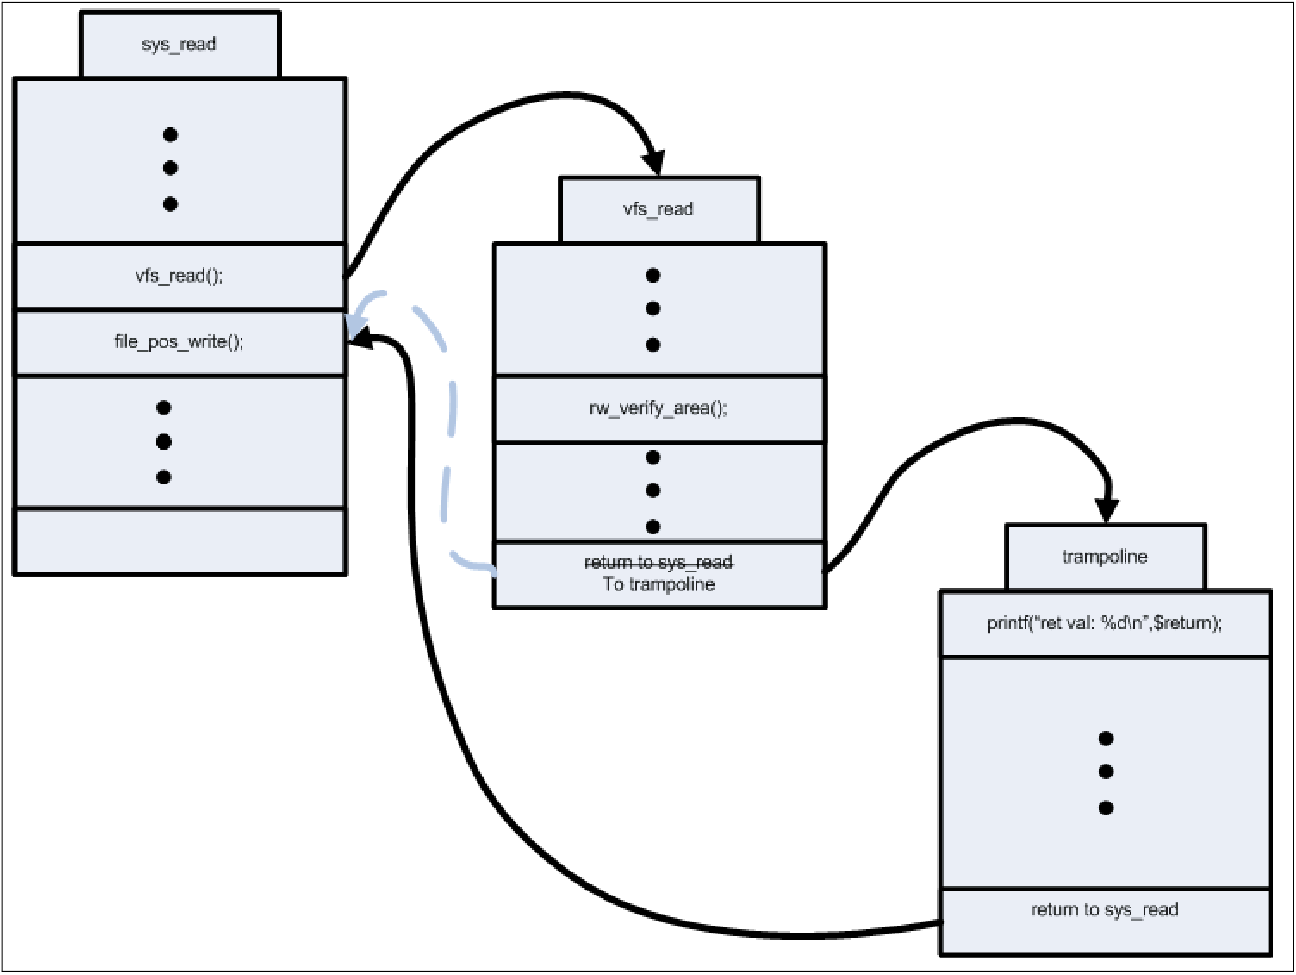
\includegraphics[scale=0.4]{attachements/kretprob.png}
	\caption{Fonctionnement tel que décrit dans la référence IBM sur Systemtap \cite{IBMRBST}}
\end{figure}

\subsubsection{Résultats obtenus}

Après s'être familiarisé avec le fonctionnement de Systemtap, nous nous sommes aperçu que les scripts utilisés pour récupérer les informations issues des appels système sont exécutés une fois l'appel système effectué. Il n'est pas possible, d'après nos recherches, de faire en sorte que les scripts puissent bloquer les appels système avant de les effectuer.

De ce fait, l'utilisation de Systemtap ne permet pas de répondre à nos besoins.

Il faut ajouter à cela que les informations recueillies à partir de Systemtap ne sont pas exploitables pour certaines d'entre-elles. Par exemple, lorsqu'un fichier est accédé (lu ou écrit), seul le numéro d'inode nous était retourné. Il n'était alors pas pertinent de récupérer le chemin complet du fichier, car cette recherche est inadaptée et inefficace : il est nécessaire de parcourir l'intégralité du système de fichiers.

Il fallait donc changer de stratégie. C'est pourquoi, nous avons, avec l'accord du responsable du projet, décidé de nous orienter vers l'utilisation des ``Linux Security Modules'' (LSM).

\subsection{Linux Security Modules}

\subsubsection{Principe de fonctionnement}

Les modules LSM sont au noyau ce que netfilter est au réseau.

Le principe de fonctionnement est simple : un module LSM est chargé dans le noyau Linux au démarrage. Il se substitue ou complète alors la procédure de contrôle d'accès. \`A chaque appel système est associé un point d'ancrage ou hook que l'on peut considérer comme une fonction. Il est placé dans l'appel système entre les vérifications élémentaires (existence des fichiers, droits unix) et sa réalisation. Dès qu'un appel système est demandé, le hook est exécuté. Par défaut, il autorise l'exécution de l'appel système.

\begin{figure}[hb]
	\centering
	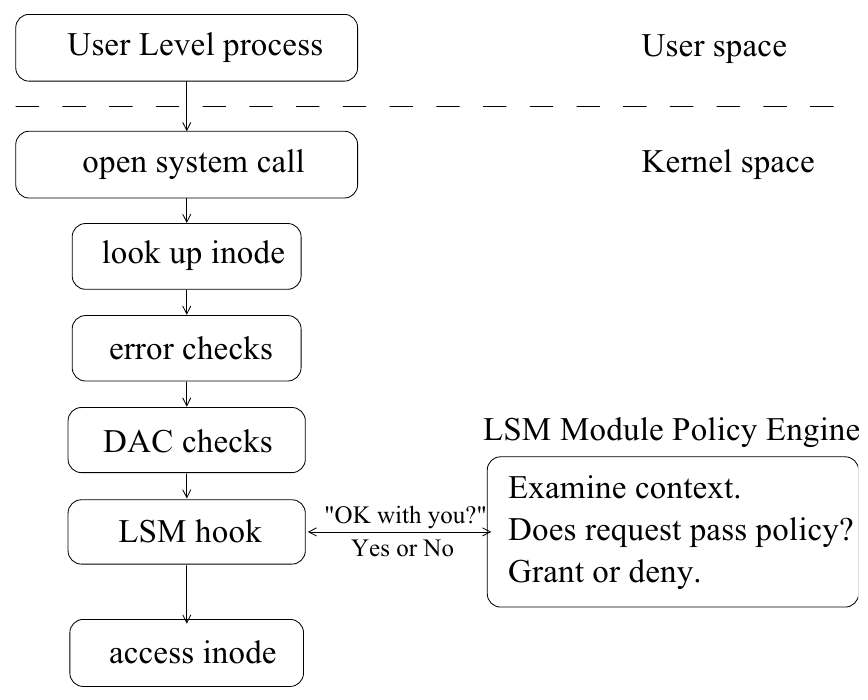
\includegraphics[scale=0.45]{attachements/lsm1.png}
	\caption{Architecture des hooks LSM \cite{LSMINTRO}}
\end{figure}

L'avantage de ces hooks est qu'ils offrent une très grande liberté. Cependant, il n'est possible pour le moment de ne charger dans le noyau qu'un seul et unique module LSM. Or, PIGA-OS utilise déjà un module LSM : SELinux.

\begin{figure}%[hb]
	\centering
	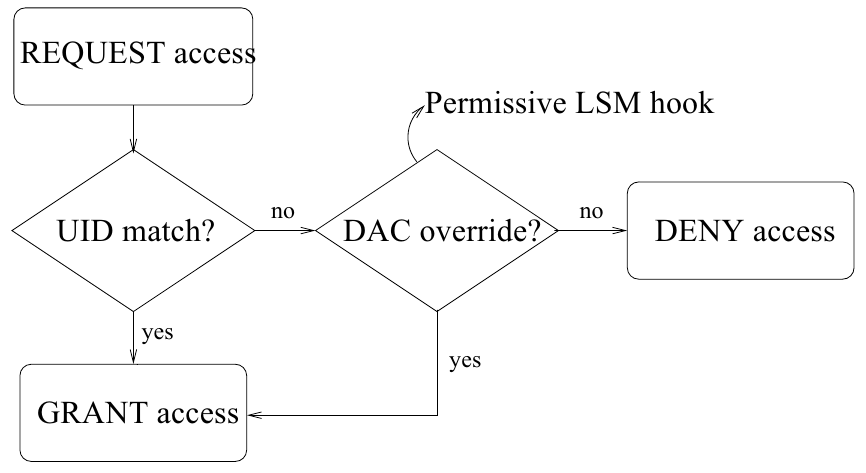
\includegraphics[scale=0.45]{attachements/lsm2.png}
	\caption{Hook LSM permissif. Ce hook autorise la politique de sécurité à passer outre les restrictions DAC \cite{LSMINTRO}}
\end{figure}

Pour les besoins du développement, nous avons dû désactiver SELinux, pour nous concentrer sur notre propre module, et non sur l'intégration avec le module LSM de SELinux.

\subsubsection{Implémentation}

Nous avons donc développé un module LSM qui "hook" les appels système. Par défaut, ces hooks sont "transparents" à l'exception du hook "file permission" sur lequel nous avons travaillé. Il est appelé à chaque ouverture (lecture, écriture, exécution) de descripteur de fichier.

Nous avons ajouté la possibilité d'activer ou non ce module lors de la compilation du noyau en suivant les conventions de nommage des options de configuration.

Nous avons également remarqué que les hooks ``socket\_bind'' et ``socket\_connect'' permetent de récupérer des informations, notamment l'adresse IP et le port de destination d'une socket, avant qu'elle ne soit créée. Ils permettent ainsi d'obtenir l'adresse IP et le port qui correspondent à une connexion. Il existe également deux autres "hooks" ``socket\_recvmsg'' et ``socket\_sendmsg'' qui permettent, eux, de pouvoir exercer un contrôle en fonction du contenu du paquet. On peut donc imaginer grâce à ces quatre "hook" pouvoir surveiller les connexions réseau.

Par manque de temps, nous avons décidé de ne pas surveiller ces "hooks". Cependant, nous avons tout mis en œuvre afin que les informations disponibles dans ces "hook" arrivent à contextd, afin, de pouvoir travailler sur l'exploitation des données et effectuer les contrôls voulus à l'avenir.

En effet, contextd ne permet pas de prendre de décisions sur les adresses IP mais seulement sur les URLs. Une requête DNS inverse ne permet malheuresement pas d'obtenir d'adresse utilisable par contextd. Nous n'avons donc pas poursuivit l'intégration des ``connexions'' dans notre solution.

La principale difficulté de cette étape fut de localiser dans quels fichiers ces informations sont définies parmi l'ensemble du code source du noyau Linux. S'agissant de structures pour la plupart, il nous fallait savoir quels en étaient les membres pour pouvoir en tirer les informations essentielles au fonctionnement de contextd.

Nous avons donc dû étudier également le fonctionnement du démon contextd. Il s'avère qu'il n'a besoin que de peu de données et se contente de :
	\begin{itemize}
		\item le PID
		\item l'execname
		\item le chemin complet du fichier
		\item le context de sécurité SELinux~\\
	\end{itemize}
	
\textit{\textsl{\textbf{Nota bene :}}} Pour les activitées réseaux, contextd à besoin de non seulement du FQDN mais aussi de la page et/ou des sous-domaines associés. Or, au niveau du noyau n'est accessible que l'adresse IP. Il faut donc pouvoir retrouver à partir de l'IP le FQDN. Après uen tentative, grâce à la fonction \textit{getnamebyaddr}, nous avons pu retrouver un FQDN exploitable. En effet, nous avons tenté une connexion vers www.google.fr afin de voir, si à partir de l'adresse IP résolue, on pouvait retrouver google. Force est de constater que le résultat, wy-in-f104.1e100.net, bien qu'il redirige vers google, n'est pas exploitable par contextd.

Maintenant que ces informations sont localisées, il faut pouvoir les extraire de l'espace noyau (kernel space) pour les acheminer dans l'espace utilisateur (User space) là où opère contextd. 

\subsection{La communication entre contextd et le noyau}

Compte tenu du fonctionnement de contextd, il a fallut développé un système de communication entre le noyau et contextd.

\begin{figure}[hb]
	\centering
	\includesvg{attachements/fonctionnement_avant}{1.6}
	\caption{Communication entre contextd et les applications}
\end{figure}

En effet, comme le montre le schéma, aucune implémentation ne permet à contextd de communiquer avec le noyau ; l'interface DBUS étant réservé historiquement qu'aux communications entre processus.

\subsubsection{Les proc files}

Pour la communication entre le noyau et l'espace utilisateur, ont été créés les proc files. Ce système de fichiers créé en RAM permet non seulement de récupéré des informations depuis le noyau mais aussi de pouvoir lui en envoyer.

Nous avons donc envisager de créer des proc files afin de pouvoir récupérer les informations utiles à contextd décrites précédemment. Cependant, il a fallu considéré les problèmes liés aux aspects sécurité. Nous avons donc décider de ne pas retenir cette idée, tout en la retenant pour le débuggage. (cf. L'interface présentée à l'administrateur).

\subsubsection{Les appels systèmes}

Pour mettre en place la communication entre l'espace noyau et le démon en espace utilisateur contextd, nous avons implémenté trois nouveaux appels systèmes. En effet, la solution des appels systèmes nous permet de contrôler les intéractions avec le noyau en créant :
\begin{itemize}
 \item \textbf{auditsec\_reg} : démarre/termine la communication et enregistre/désinscrit les programmes à surveiller.
 \item \textbf{auditsec\_question} : bloquant, qui attends une demande d'autorisation de la part du noyau.
 \item \textbf{auditsec\_answer} : qui permet de donner une réponse au noyau.
\end{itemize}

\begin{figure}[hb]
	\centering
	\includepic{attachements/sequence_diagram}{1}
	\caption{Diagramme de séquence entre le noyau et contextd}
\end{figure}

Nous utilisons des mutex pour contrôler les échanges d'informations entre le noyau et le démon et de s'assurer le traitement de chacun des appels système.

\begin{figure}[hb]
	\centering
	\includesvg{attachements/syscall_sync}{0.6}
	\caption{Communication entre les hooks LSM et les appels système}
\end{figure}

% FIXME
L'appel système "auditsec\_reg" qui permet à contextd de se faire connaître du noyau n'est pas tout à fait sûr. En effet, il n'est pas exclu qu'un program malveillant puisse s'enregistrer auprès du noyau via cet appel système sans que ce soit contextd. Une solution d'enregistrement sécurisé et sûre est à envisager à l'avenir.
% FIXME

\subsubsection{L'interface présentée à l'administrateur}

	Pour faciliter l'administration et pour pouvoir intéragir plus aisément avec le noyau, nous avons mis en place deux "proc files" :

	\begin{itemize}
		\item /proc/contextd/programs : Ce fichier liste les programmes qui ont été enregistrés auprès du noyau et qui sont donc surveillés. Ce fichier n'est disponible qu'en lecture seule afin de ne pas permettre un acte malveillant consistant à ajouter ou supprimer un programme de manière intempestive.
		\item /proc/contextd/status : Ce fichier est en revanche accessible en lecture/écriture. En lecture, il renvoie le PID de contextd (plus précisément le tgid (threads)). En ecriture, s'il reçoit un 0, il désactive la surveillance des programmes enregistrés et vide la liste.
	\end{itemize}


\subsection{Intéractions entre un processus, le noyau et contextd}

Compte tenu de ce qui a été précédemment dit, nous avons dû modifier contextd afin de lui ajouter la possibilité de communiquer avec les processus via le noyau. Pour ce faire, nous nous sommes inspirés de ce qui était déjà implémenté, à savoir la communication par un canal dbus.

\subsection{Ajouts à contextd}

\subsubsection{Classes de communication}

Cette communication se faisait grâce à la classe "dbus-context". Cette classe traitait les solicitations des clients (programmes), les enregistrait dans une liste (attribut privé) et s'occupait des transitions, cette liste (Qmap) était indexée par le dbus\_id.

Nous avons donc fait la même chose pour le noyau. Nous avons créé une classe "kernel-context" qui permet de traiter les autres processus qui ne disposent pas du plugin. Cependant, il faut tenir compte du fait que dans ce cas de figure, une application qui possède le plugin se verra authentifiée deux fois, une fois par dbus et une fois par le noyau. De plus, la liste des processus ne peut plus être indexée par le dbus\_id car il n'est pas pertinent dans le cas du noyau.

Pour palier ce problème, nous avons décidé d'implémenter une classe abstraite "abstractcontext" qui, elle, possède une seule et unique liste qui contiendra les clients des deux modes de communication, à savoir dbus et noyau tous deux étant implémentées respectivement par "dbus-context" et "kernel-context", classes dérivées de "abstractcontext". Dans le cas où un troisième mode de communication sera envisagé, il sera alors aisé de faire les modifications pour que celui-ci s'intègre parfaitement à ce qui existe déjà. La liste en question est déclarée en private static : ces propriétés permettent à toutes les classes dérivées d'hériter de l'instanciation de cette liste sans que celle-ci dépende de l'instance.

De même, pour lire cette liste, ajouter ou supprimer un élément, on utilise un vérrou (lock) afin d'éviter les accès concurrents. Ce vérrou est également déclaré en protected static, pour les mêmes raison évoquées supra concernant l'héritage et l'instanciation.

\begin{figure}[h]
	\centering
	\includedot{attachements/class}{.8}
	\caption{Diagramme de classes}
\end{figure}

\subsubsection{Surveillance et enregistrement dynamique}

Pour rendre contextd conscient de nos modifications nous avons implémenté plusieurs éléments :

\begin{itemize}
	\item L'enregistrement et la désinscription/mise à jour de la liste des programmes surveillés par contextd lors de la réception du signal SIGUSR2.
	\item La vérification de la cohérence de la liste des clients stockée par contextd : cette liste est maintenant nettoyée à intervalles réguliers.
\end{itemize}

De plus, notre solution nécessitant maintenant l'enregistrement des programmes auprès du noyau, il est désormé possible de charger dynamique cette liste de programmes à partir de /etc/context.d/program.d. Il est par contre nécessaire de préciser à contextd, à la compilation, les programmes à exclure de cette liste (pour l'instant firefox, claws-mail et context-notify).

\textit{\textsl{\textbf{Nota bene :}}} Nous partons du principe que notre travail est/sera utilisé avec SELinux, même s'il ce n'est pas possible actuellement. Nous n'effectuons aucune vérification d'intégrité sur les programmes surveillés par contextd. Cette intégrité est en principe assurée par les politiques SELinux et/ou les règles PIGA.

%Notre travail dépendant intégralement des solutions sous-jacentes.

\subsection{Résultats finaux}

Le produit de notre travail correspond globalement à ce qui était attendu. En effet, nos tests effectués à l'aide d'un programme de test "testprog" montrent que le comportement du système est bien celui attendu. Lorsque ce programme de test tente d'ouvrir un fichier qui appartient à un autre domaine que le domaine actuel, si la transaction est autorisée, une demande de changement de domaine est envoyé à context-notify qui attend la réponse, sinon, la demande est rejetée.

D'autres tests effectués avec Libreoffice, montre que le résultat fonctionne parfaitement avec des programmes classiques et courant sans aucune modification. Cependant, les erreurs affichées par ces applications ne sont pas forcément très explicites (Libreoffice considère parfois que le document est endommagé alors que le noyau lui a tout simplement refusé l'accès). Ce problème est lié au choix de LSM, les applications ne pouvant faire la différence entre un refus lié aux permissions classiques par rapport au refus lié au module de sécurité. Ces mêmes cas de figure se produisent sur un système utilisant SELinux, lors des refus de transitions de contexte.

\begin{figure}[h]
	\centering
	\includesvg{attachements/fonctionnement_apres}{1.3}
	\caption{Schéma des classes}
\end{figure}

\subsection{Améliorations possibles et remarques}
	\begin{itemize}
		\item Les règles (regexp) des fichiers filtrés deviennent très compliquées car il faut autoriser toutes les librairies pour les programmes non compilés en statique.
		\item Intégré les hook à SELinux. En effet, pour le moment, seul un module LSM est chargeable au niveau du noyau. Il n'est donc pas possible de déployer notre solution en cohabitation avec SELinux.
	\end{itemize}

\newpage

\section{Résultats et benchmarks}

Benchmark : Sans le module LSM, Avec le module mais pas lancé, Avec le module et lancé

\newpage

\section*{Conclusion} \addcontentsline{toc}{section}{Conclusion}

Le but de ce projet était de simplifier l'ajout d'application à PIGA-SYSTRANS et au système PIGA-OS. Cet objectif est atteint car nos travaux permettent, par exemple, de faire fonctionner OpenOffice.org/LibreOffice avec contextd, sans modifier ces applications.

De plus, l'aspect totalement générique de notre solution nous assure un fort potentiel de réutilisation. En effet, les ajouts dans contextd permmettant le chargement dynamique de programmes à contrôler nous permettent de se concentrer sur l'écriture de règles contextd, et non sur la modification des applications. Il ne reste alors plus qu'à modifier uniquement les applications possédant un comportment s'étendant sur plusieurs domaines et dont l'état interne nécessite des modifications lors d'un changement de domaine.

TODO Remarques sur SELinux / intégration avec PIGA-OS ...

% Le retard, sur la partie implémentation noyau, par rapport à notre planification est principalement dû à notre découverte très progressive des capacités offertes aux développeurs. Le livre Linux Kernel Development \cite{LKDTE} nous a permis de faire un bon en avant dans la compréhension du fonctionnement du noyau et notamment l'implémentation des appels système.

\newpage
% \addcontentsline{toc}{section}{Annexes}
\addcontentsline{toc}{section}{Références}

% \subsection*{Liens et références}
\begin{thebibliography}{40}

\bibitem{IBMRBST} \textit{IBM Redbooks : SystemTap: Instrumenting the Linux Kernel for Analyzing Performance and Functional Problems}, Bart Jacob, Paul Larson, Breno Henrique Leitao, Saulo Augusto M Martins da Silva, \url{http://www.redbooks.ibm.com/abstracts/redp4469.html}

\bibitem{LSMINTRO} \textit{Linux Security Modules : General Security Support for the Linux Kernel}, Chris Wright, Crispin Cowan, Stephen Smalley, James Morris, Greg Kroah-Hartman, \url{http://citeseerx.ist.psu.edu/viewdoc/download?doi=10.1.1.84.6867&rep=rep1&type=pdf}

\bibitem{LKDSE} \textit{Linux Kernel Development, Second Edition}, Robert Love, Novell Press
\bibitem{LKDTE} \textit{Linux Kernel Development, Third Edition}, Robert Love, Pearson Education, Inc.

\bibitem{MRHEL5} \textit{Managing Red Hat Enterprise Linux 5}, Daniel J Walsh, Karl MacMillan, \url{http://people.redhat.com/dwalsh/SELinux/Presentations/ManageRHEL5.pdf}

\bibitem{WCS} \textit{Wikipedia : Computer Security}, \url{http://en.wikipedia.org/wiki/Computer_security}

\bibitem{SOURCE} Code source (kernel 2.6.32 hardened r22, piga-systrans, et scripts systemtap) disponible sur le serveur de projet STI (le projet s'appelle Contextd Capture), \url{http://projetsti.ensi-bourges.fr/projects/promo2012-systemtap}.

\bibitem{TIOF} P...

\bibitem{QNX} QNX Realtime Operating System, \url{http://www.qnx.com}

\end{thebibliography}

%\printindex

\end{document}